% Options for packages loaded elsewhere
\PassOptionsToPackage{unicode}{hyperref}
\PassOptionsToPackage{hyphens}{url}
%
\documentclass[
]{article}
\usepackage{lmodern}
\usepackage{amssymb,amsmath}
\usepackage{ifxetex,ifluatex}
\ifnum 0\ifxetex 1\fi\ifluatex 1\fi=0 % if pdftex
  \usepackage[T1]{fontenc}
  \usepackage[utf8]{inputenc}
  \usepackage{textcomp} % provide euro and other symbols
\else % if luatex or xetex
  \usepackage{unicode-math}
  \defaultfontfeatures{Scale=MatchLowercase}
  \defaultfontfeatures[\rmfamily]{Ligatures=TeX,Scale=1}
\fi
% Use upquote if available, for straight quotes in verbatim environments
\IfFileExists{upquote.sty}{\usepackage{upquote}}{}
\IfFileExists{microtype.sty}{% use microtype if available
  \usepackage[]{microtype}
  \UseMicrotypeSet[protrusion]{basicmath} % disable protrusion for tt fonts
}{}
\makeatletter
\@ifundefined{KOMAClassName}{% if non-KOMA class
  \IfFileExists{parskip.sty}{%
    \usepackage{parskip}
  }{% else
    \setlength{\parindent}{0pt}
    \setlength{\parskip}{6pt plus 2pt minus 1pt}}
}{% if KOMA class
  \KOMAoptions{parskip=half}}
\makeatother
\usepackage{xcolor}
\IfFileExists{xurl.sty}{\usepackage{xurl}}{} % add URL line breaks if available
\IfFileExists{bookmark.sty}{\usepackage{bookmark}}{\usepackage{hyperref}}
\hypersetup{
  pdftitle={Supplementary Material for: A Rough Guide to Pre-processing High-Frequency Animal Tracking Data},
  pdfauthor={Pratik R. Gupte; Christine E. Beardsworth; Orr Spiegel; Emmanuel Lourie; Allert Bijleveld},
  hidelinks,
  pdfcreator={LaTeX via pandoc}}
\urlstyle{same} % disable monospaced font for URLs
\usepackage[left=4cm, right=3cm, top=2.5cm, bottom=2.5cm]{geometry}
\usepackage{color}
\usepackage{fancyvrb}
\newcommand{\VerbBar}{|}
\newcommand{\VERB}{\Verb[commandchars=\\\{\}]}
\DefineVerbatimEnvironment{Highlighting}{Verbatim}{commandchars=\\\{\}}
% Add ',fontsize=\small' for more characters per line
\newenvironment{Shaded}{}{}
\newcommand{\AlertTok}[1]{\textcolor[rgb]{1.00,0.00,0.00}{\textbf{#1}}}
\newcommand{\AnnotationTok}[1]{\textcolor[rgb]{0.38,0.63,0.69}{\textbf{\textit{#1}}}}
\newcommand{\AttributeTok}[1]{\textcolor[rgb]{0.49,0.56,0.16}{#1}}
\newcommand{\BaseNTok}[1]{\textcolor[rgb]{0.25,0.63,0.44}{#1}}
\newcommand{\BuiltInTok}[1]{#1}
\newcommand{\CharTok}[1]{\textcolor[rgb]{0.25,0.44,0.63}{#1}}
\newcommand{\CommentTok}[1]{\textcolor[rgb]{0.38,0.63,0.69}{\textit{#1}}}
\newcommand{\CommentVarTok}[1]{\textcolor[rgb]{0.38,0.63,0.69}{\textbf{\textit{#1}}}}
\newcommand{\ConstantTok}[1]{\textcolor[rgb]{0.53,0.00,0.00}{#1}}
\newcommand{\ControlFlowTok}[1]{\textcolor[rgb]{0.00,0.44,0.13}{\textbf{#1}}}
\newcommand{\DataTypeTok}[1]{\textcolor[rgb]{0.56,0.13,0.00}{#1}}
\newcommand{\DecValTok}[1]{\textcolor[rgb]{0.25,0.63,0.44}{#1}}
\newcommand{\DocumentationTok}[1]{\textcolor[rgb]{0.73,0.13,0.13}{\textit{#1}}}
\newcommand{\ErrorTok}[1]{\textcolor[rgb]{1.00,0.00,0.00}{\textbf{#1}}}
\newcommand{\ExtensionTok}[1]{#1}
\newcommand{\FloatTok}[1]{\textcolor[rgb]{0.25,0.63,0.44}{#1}}
\newcommand{\FunctionTok}[1]{\textcolor[rgb]{0.02,0.16,0.49}{#1}}
\newcommand{\ImportTok}[1]{#1}
\newcommand{\InformationTok}[1]{\textcolor[rgb]{0.38,0.63,0.69}{\textbf{\textit{#1}}}}
\newcommand{\KeywordTok}[1]{\textcolor[rgb]{0.00,0.44,0.13}{\textbf{#1}}}
\newcommand{\NormalTok}[1]{#1}
\newcommand{\OperatorTok}[1]{\textcolor[rgb]{0.40,0.40,0.40}{#1}}
\newcommand{\OtherTok}[1]{\textcolor[rgb]{0.00,0.44,0.13}{#1}}
\newcommand{\PreprocessorTok}[1]{\textcolor[rgb]{0.74,0.48,0.00}{#1}}
\newcommand{\RegionMarkerTok}[1]{#1}
\newcommand{\SpecialCharTok}[1]{\textcolor[rgb]{0.25,0.44,0.63}{#1}}
\newcommand{\SpecialStringTok}[1]{\textcolor[rgb]{0.73,0.40,0.53}{#1}}
\newcommand{\StringTok}[1]{\textcolor[rgb]{0.25,0.44,0.63}{#1}}
\newcommand{\VariableTok}[1]{\textcolor[rgb]{0.10,0.09,0.49}{#1}}
\newcommand{\VerbatimStringTok}[1]{\textcolor[rgb]{0.25,0.44,0.63}{#1}}
\newcommand{\WarningTok}[1]{\textcolor[rgb]{0.38,0.63,0.69}{\textbf{\textit{#1}}}}
\usepackage{longtable,booktabs}
% Correct order of tables after \paragraph or \subparagraph
\usepackage{etoolbox}
\makeatletter
\patchcmd\longtable{\par}{\if@noskipsec\mbox{}\fi\par}{}{}
\makeatother
% Allow footnotes in longtable head/foot
\IfFileExists{footnotehyper.sty}{\usepackage{footnotehyper}}{\usepackage{footnote}}
\makesavenoteenv{longtable}
\usepackage{graphicx}
\makeatletter
\def\maxwidth{\ifdim\Gin@nat@width>\linewidth\linewidth\else\Gin@nat@width\fi}
\def\maxheight{\ifdim\Gin@nat@height>\textheight\textheight\else\Gin@nat@height\fi}
\makeatother
% Scale images if necessary, so that they will not overflow the page
% margins by default, and it is still possible to overwrite the defaults
% using explicit options in \includegraphics[width, height, ...]{}
\setkeys{Gin}{width=\maxwidth,height=\maxheight,keepaspectratio}
% Set default figure placement to htbp
\makeatletter
\def\fps@figure{htbp}
\makeatother
\setlength{\emergencystretch}{3em} % prevent overfull lines
\providecommand{\tightlist}{%
  \setlength{\itemsep}{0pt}\setlength{\parskip}{0pt}}
\setcounter{secnumdepth}{2}

\usepackage{fontspec}
% use nice fonts if available else use boring defaults

\usepackage{lineno}
\setmainfont{Times New Roman}

\linenumbers
\newlength{\cslhangindent}
\setlength{\cslhangindent}{1.5em}
\newenvironment{cslreferences}%
  {\setlength{\parindent}{0pt}%
  \everypar{\setlength{\hangindent}{\cslhangindent}}\ignorespaces}%
  {\par}

\title{Supplementary Material for: A Rough Guide to Pre-processing High-Frequency Animal Tracking Data}
\author{Pratik R. Gupte \and Christine E. Beardsworth \and Orr Spiegel \and Emmanuel Lourie \and Allert Bijleveld}
\date{2020-11-16}

\begin{document}
\maketitle

{
\setcounter{tocdepth}{2}
\tableofcontents
}
\hypertarget{processing-egyptian-fruit-bat-tracks}{%
\section{Processing Egyptian fruit bat tracks}\label{processing-egyptian-fruit-bat-tracks}}

We show the pre-processing pipeline at work on the tracks of three Egyptian fruit bats (\emph{Rousettus aegyptiacus}), and construct residence patches.

\hypertarget{prepare-libraries}{%
\subsection{Prepare libraries}\label{prepare-libraries}}

Install the required \texttt{R} libraries that are available on CRAN.

\begin{Shaded}
\begin{Highlighting}[]
\CommentTok{\# load libs}
\KeywordTok{library}\NormalTok{(data.table)}
\KeywordTok{library}\NormalTok{(RSQLite)}
\KeywordTok{library}\NormalTok{(ggplot2)}
\KeywordTok{library}\NormalTok{(patchwork)}

\CommentTok{\# prepare a palette}
\NormalTok{pal <{-}}\StringTok{ }\NormalTok{RColorBrewer}\OperatorTok{::}\KeywordTok{brewer.pal}\NormalTok{(}\DecValTok{4}\NormalTok{, }\StringTok{"Set1"}\NormalTok{)}
\end{Highlighting}
\end{Shaded}

\hypertarget{install-atlastools-from-github.}{%
\subsection{\texorpdfstring{Install \texttt{atlastools} from Github.}{Install atlastools from Github.}}\label{install-atlastools-from-github.}}

\texttt{atlastools} is available from Github and is archived on Zenodo (Gupte \protect\hyperlink{ref-gupte2020a}{2020}).
It can be installed using \texttt{remotes} or \texttt{devtools}. Here we use the \texttt{remotes} function \texttt{install\_github}.

\begin{Shaded}
\begin{Highlighting}[]
\KeywordTok{install.packages}\NormalTok{(}\StringTok{"remotes"}\NormalTok{)}

\CommentTok{\# installation using remotes}
\NormalTok{remotes}\OperatorTok{::}\KeywordTok{install\_github}\NormalTok{(}\StringTok{"pratikunterwegs/atlastools"}\NormalTok{)}
\end{Highlighting}
\end{Shaded}

\hypertarget{read-bat-data}{%
\subsection{Read bat data}\label{read-bat-data}}

Read the bat data from an \texttt{SQLite} database local file and convert to a plain text csv file.
This data can be found in the ``data'' folder.

\begin{Shaded}
\begin{Highlighting}[]
\CommentTok{\# prepare the connection}
\NormalTok{con <{-}}\StringTok{ }\KeywordTok{dbConnect}\NormalTok{(}\DataTypeTok{drv =} \KeywordTok{SQLite}\NormalTok{(), }
                 \DataTypeTok{dbname =} \StringTok{"data/Three\_example\_bats.sql"}\NormalTok{)}

\CommentTok{\# list the tables}
\NormalTok{table\_name <{-}}\StringTok{ }\KeywordTok{dbListTables}\NormalTok{(con)}

\CommentTok{\# prepare to query all tables}
\NormalTok{query <{-}}\StringTok{ }\KeywordTok{sprintf}\NormalTok{(}\StringTok{\textquotesingle{}select * from }\CharTok{\textbackslash{}"}\StringTok{\%s}\CharTok{\textbackslash{}"}\StringTok{\textquotesingle{}}\NormalTok{, table\_name)}

\CommentTok{\# query the database}
\NormalTok{data <{-}}\StringTok{ }\KeywordTok{dbGetQuery}\NormalTok{(}\DataTypeTok{conn =}\NormalTok{ con, }\DataTypeTok{statement =}\NormalTok{ query)}

\CommentTok{\# disconnect from database}
\KeywordTok{dbDisconnect}\NormalTok{(con)}
\end{Highlighting}
\end{Shaded}

Convert data to csv, and save a local copy in the folder ``data''.

\begin{Shaded}
\begin{Highlighting}[]
\CommentTok{\# convert data to datatable}
\KeywordTok{setDT}\NormalTok{(data)}

\CommentTok{\# write data for QGIS}
\KeywordTok{fwrite}\NormalTok{(data, }\DataTypeTok{file =} \StringTok{"data/bat\_data.csv"}\NormalTok{)}
\end{Highlighting}
\end{Shaded}

\hypertarget{a-first-visual-inspection}{%
\subsection{A First Visual Inspection}\label{a-first-visual-inspection}}

Plot the bat data as a sanity check, and inspect it visually for errors (Figure 1).
The plot code is hidden in the rendered copy (PDF) of this supplementary material, but is available in the \texttt{Rmarkdown} file ``06\_bat\_data.Rmd''.
The saved plot is shown below as Figure 1.

\begin{figure}
\centering
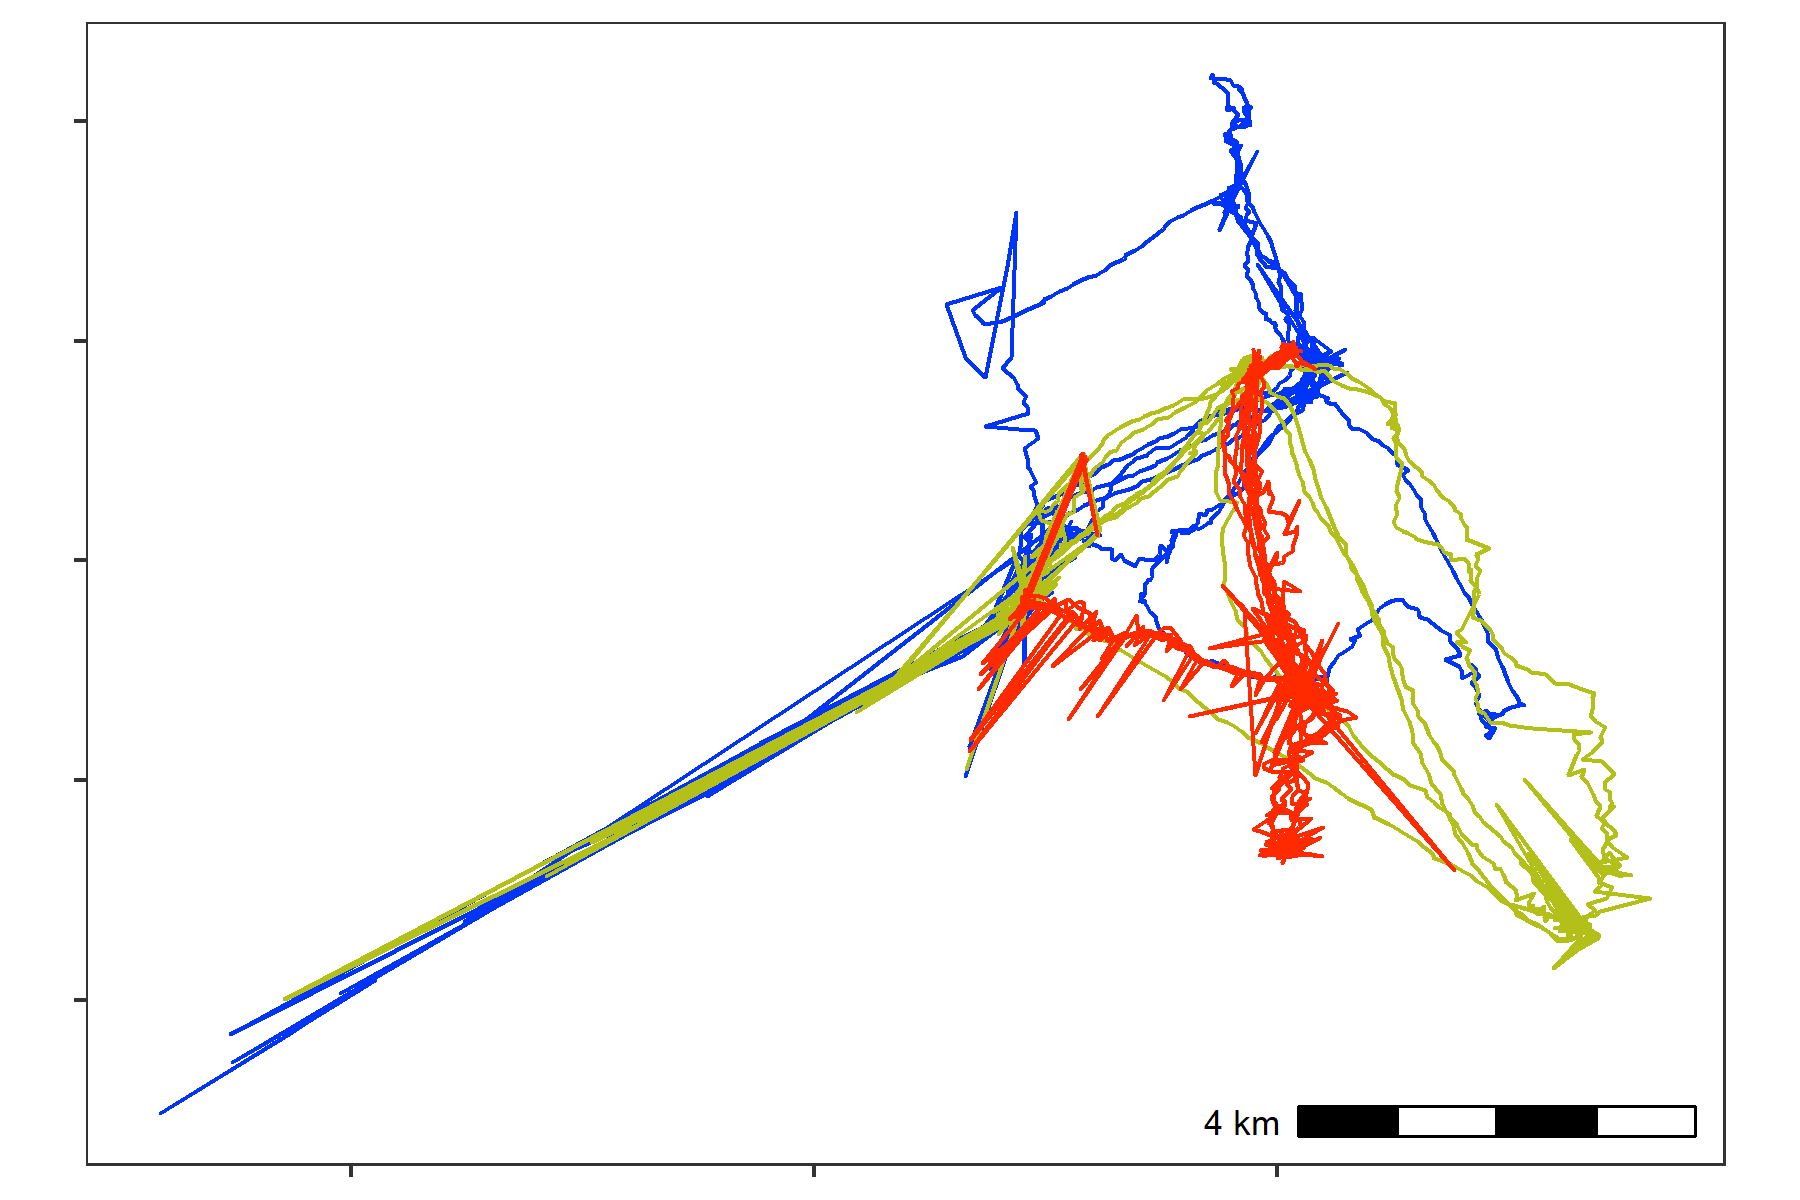
\includegraphics{figures/fig_bat_raw.png}
\caption{Movement data from three Egyptian fruit bats tracked using the ATLAS system (\emph{Rousettus aegyptiacus}; (Toledo et al. \protect\hyperlink{ref-toledo2020}{2020}; Shohami and Nathan \protect\hyperlink{ref-shohami2020}{2020})).
The bats were tracked in the Hula Valley, Israel (33.1\(^{\circ}\)N, 35.6\(^{\circ}\)E), and we use three nights of tracking (5\textsuperscript{th}, 6\textsuperscript{th}, and 7\textsuperscript{th} May, 2018), for our demonstration, with an average of 13,370 positions (SD = 2,173; range = 11,195 -- 15,542; interval = 8 seconds) per individual.
After first plotting the individual tracks, we notice severe distortions, making pre-processing necesary}
\end{figure}

\hypertarget{prepare-data-for-filtering}{%
\subsection{Prepare data for filtering}\label{prepare-data-for-filtering}}

Here we apply a series of simple filters.
It is always safer to deal with one individual at a time, so we split the data.table
into a list of data.tables to avoid mixups among individuals.

\hypertarget{prepare-data-per-individual}{%
\subsubsection{Prepare data per individual}\label{prepare-data-per-individual}}

\begin{Shaded}
\begin{Highlighting}[]
\CommentTok{\# split bat data by tag}
\CommentTok{\# first make a copy using the data.table function copy}
\CommentTok{\# this prevents the orignal data from being modified by atlastools}
\CommentTok{\# functions which DO MODIFY BY REFERENCE!}
\NormalTok{data\_split <{-}}\StringTok{ }\KeywordTok{copy}\NormalTok{(data)}

\CommentTok{\# now split}
\NormalTok{data\_split <{-}}\StringTok{ }\KeywordTok{split}\NormalTok{(data\_split, }\DataTypeTok{by =} \StringTok{"TAG"}\NormalTok{)}
\end{Highlighting}
\end{Shaded}

\hypertarget{filter-by-covariates}{%
\subsection{Filter by covariates}\label{filter-by-covariates}}

No natural bounds suggest themselves, so instead we proceed to filter by covariates, since point outliers are obviously visible.

We use filter out positions with \texttt{SD\ \textgreater{}\ 20} and positions calculated using only 3 base stations, using the function \texttt{atl\_filter\_covariates}.

First we calculate the variable \texttt{SD}.

\begin{Shaded}
\begin{Highlighting}[]
\CommentTok{\# get SD.}
\CommentTok{\# since the data are data.tables, no assignment is necessary}
\KeywordTok{invisible}\NormalTok{(}
  \KeywordTok{lapply}\NormalTok{(data\_split, }\ControlFlowTok{function}\NormalTok{(dt) \{}
\NormalTok{    dt[, SD }\OperatorTok{:}\ErrorTok{=}\StringTok{ }\KeywordTok{sqrt}\NormalTok{(VARX }\OperatorTok{+}\StringTok{ }\NormalTok{VARY }\OperatorTok{+}\StringTok{ }\NormalTok{(}\DecValTok{2} \OperatorTok{*}\StringTok{ }\NormalTok{COVXY))]}
\NormalTok{  \})}
\NormalTok{)}
\end{Highlighting}
\end{Shaded}

Then we pass the filters to \texttt{atl\_filter\_covariates}.
We apply the filter to each individual's data using an \texttt{lapply}.

\begin{Shaded}
\begin{Highlighting}[]
\CommentTok{\# filter for SD <= 20}
\CommentTok{\# here, reassignment is necessary as rows are being removed}
\CommentTok{\# the atl\_filter\_covariates function could have been used here}
\NormalTok{data\_split <{-}}\StringTok{ }\KeywordTok{lapply}\NormalTok{(data\_split, }\ControlFlowTok{function}\NormalTok{(dt) \{}
  
\NormalTok{  dt <{-}}\StringTok{ }\KeywordTok{atl\_filter\_covariates}\NormalTok{(}
    \DataTypeTok{data =}\NormalTok{ dt,}
    \DataTypeTok{filters =} \KeywordTok{c}\NormalTok{(}\StringTok{"SD <= 20"}\NormalTok{,}
                \StringTok{"NBS > 3"}\NormalTok{)}
    
\NormalTok{  )}
\NormalTok{\})}
\end{Highlighting}
\end{Shaded}

\hypertarget{sanity-check-plot-filtered-data}{%
\subsubsection{Sanity check: Plot filtered data}\label{sanity-check-plot-filtered-data}}

We plot the data to check whether the filtering has improved the data (Figure 2).
The plot code is once again hidden in this rendering, but is available in the source code file.

\begin{figure}
\centering
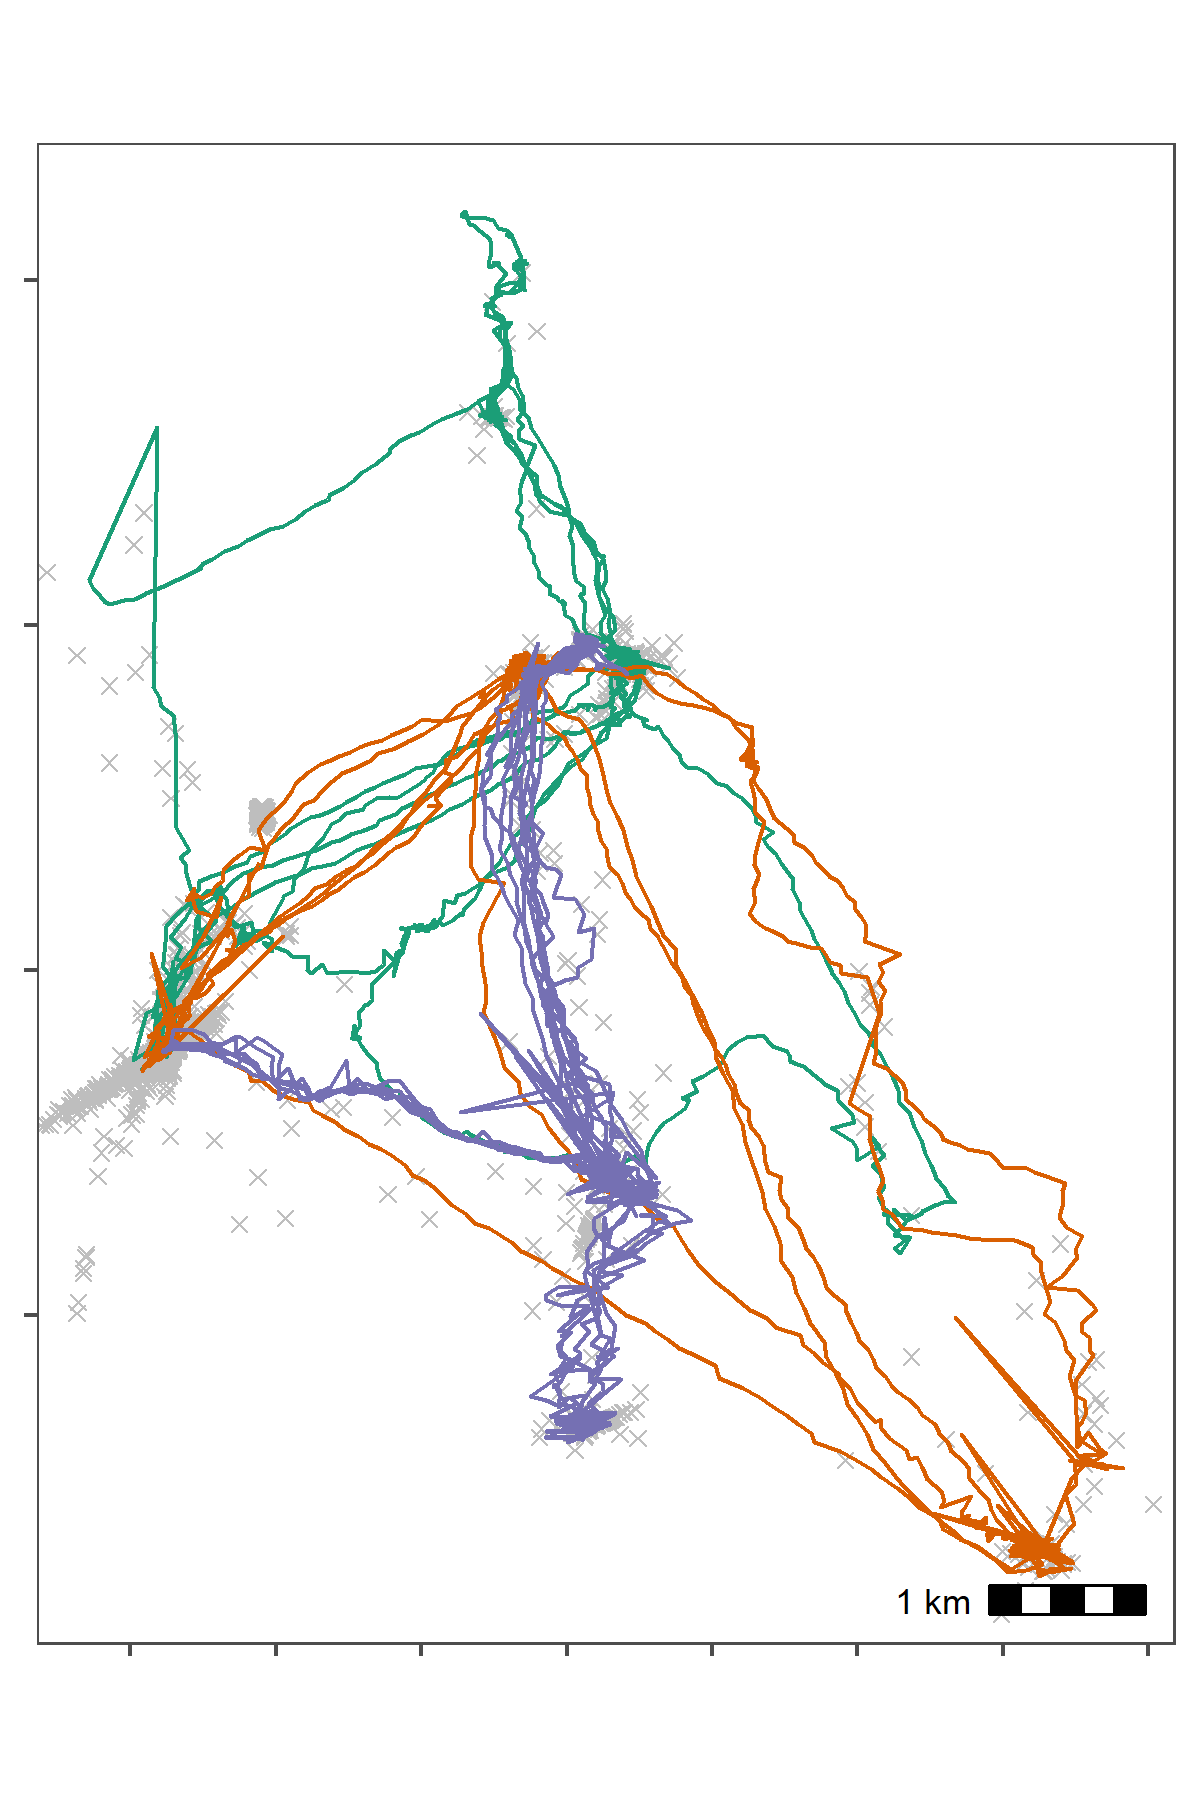
\includegraphics{figures/fig_bat_filter_cov.png}
\caption{Bat data filtered for large location errors, removing observations with standard deviation \(>\) 20. Grey crosses show data that were removed. Since the number of base stations used in the location process is a good indicator of error (Weiser et al. \protect\hyperlink{ref-weiser2016}{2016}), we also removed observations calculated using fewer than four base stations. Both steps used the function \texttt{atl\_filter\_covariates}.
This filtering reduced the data to an average of 10,447 positions per individual (78\% of the raw data on average). However, some point outliers remain.}
\end{figure}

\hypertarget{filter-by-speed}{%
\subsection{Filter by speed}\label{filter-by-speed}}

Some point outliers remain (Figure 2), and could be removed using a speed filter.

First we calculate speeds, using \texttt{atl\_get\_speed}. We must assign the speed output to a new column in the data.table, which has a special syntax which modifies in place, and is shown below. This syntax is a feature of the \texttt{data.table} package, not strictly of \texttt{atlastools} (Dowle and Srinivasan \protect\hyperlink{ref-dowle2020}{2020}).

\begin{Shaded}
\begin{Highlighting}[]
\CommentTok{\# get speeds as with SD, no reassignment required for columns}
\KeywordTok{invisible}\NormalTok{(}
  \KeywordTok{lapply}\NormalTok{(data\_split, }\ControlFlowTok{function}\NormalTok{(dt) \{}
    
    \CommentTok{\# first process time to seconds}
    \CommentTok{\# assign to a new column}
\NormalTok{    dt[, time }\OperatorTok{:}\ErrorTok{=}\StringTok{ }\KeywordTok{floor}\NormalTok{(TIME }\OperatorTok{/}\StringTok{ }\DecValTok{1000}\NormalTok{)]}
    
\NormalTok{    dt[, }\StringTok{\textasciigrave{}}\DataTypeTok{:=}\StringTok{\textasciigrave{}}\NormalTok{(}\DataTypeTok{speed\_in =} \KeywordTok{atl\_get\_speed}\NormalTok{(dt, }
                                       \DataTypeTok{x =} \StringTok{"X"}\NormalTok{, }\DataTypeTok{y =} \StringTok{"Y"}\NormalTok{, }
                                       \DataTypeTok{time =} \StringTok{"time"}\NormalTok{,}
                                       \DataTypeTok{type =} \StringTok{"in"}\NormalTok{),}
              \DataTypeTok{speed\_out =} \KeywordTok{atl\_get\_speed}\NormalTok{(dt, }
                                       \DataTypeTok{x =} \StringTok{"X"}\NormalTok{, }\DataTypeTok{y =} \StringTok{"Y"}\NormalTok{, }
                                       \DataTypeTok{time =} \StringTok{"time"}\NormalTok{,}
                                       \DataTypeTok{type =} \StringTok{"out"}\NormalTok{))]}
\NormalTok{  \})}
\NormalTok{)}
\end{Highlighting}
\end{Shaded}

Now filter for speeds \textgreater{} 20 m/s (around 70 km/h), passing the predicate (a statement return TRUE or FALSE) to \texttt{atl\_filter\_covariates}. First, we remove positions which have \texttt{NA} for their \texttt{speed\_in} (the first position) and their \texttt{speed\_out} (last position).

\begin{Shaded}
\begin{Highlighting}[]
\CommentTok{\# filter speeds}
\CommentTok{\# reassignment is required here}
\NormalTok{data\_split <{-}}\StringTok{ }\KeywordTok{lapply}\NormalTok{(data\_split, }\ControlFlowTok{function}\NormalTok{(dt) \{}
\NormalTok{  dt <{-}}\StringTok{ }\KeywordTok{na.omit}\NormalTok{(dt, }\DataTypeTok{cols =} \KeywordTok{c}\NormalTok{(}\StringTok{"speed\_in"}\NormalTok{, }\StringTok{"speed\_out"}\NormalTok{))}
  
\NormalTok{  dt <{-}}\StringTok{ }\KeywordTok{atl\_filter\_covariates}\NormalTok{(}\DataTypeTok{data =}\NormalTok{ dt,}
                              \DataTypeTok{filters =} \KeywordTok{c}\NormalTok{(}\StringTok{"speed\_in <= 20"}\NormalTok{,}
                                          \StringTok{"speed\_out <= 20"}\NormalTok{))}
\NormalTok{\})}
\end{Highlighting}
\end{Shaded}

\hypertarget{sanity-check-plot-speed-filtered-data}{%
\subsubsection{Sanity check: Plot speed filtered data}\label{sanity-check-plot-speed-filtered-data}}

The speed filtered data is now inspected for errors (Figure 3). The plot code is once again hidden.

\begin{figure}
\centering
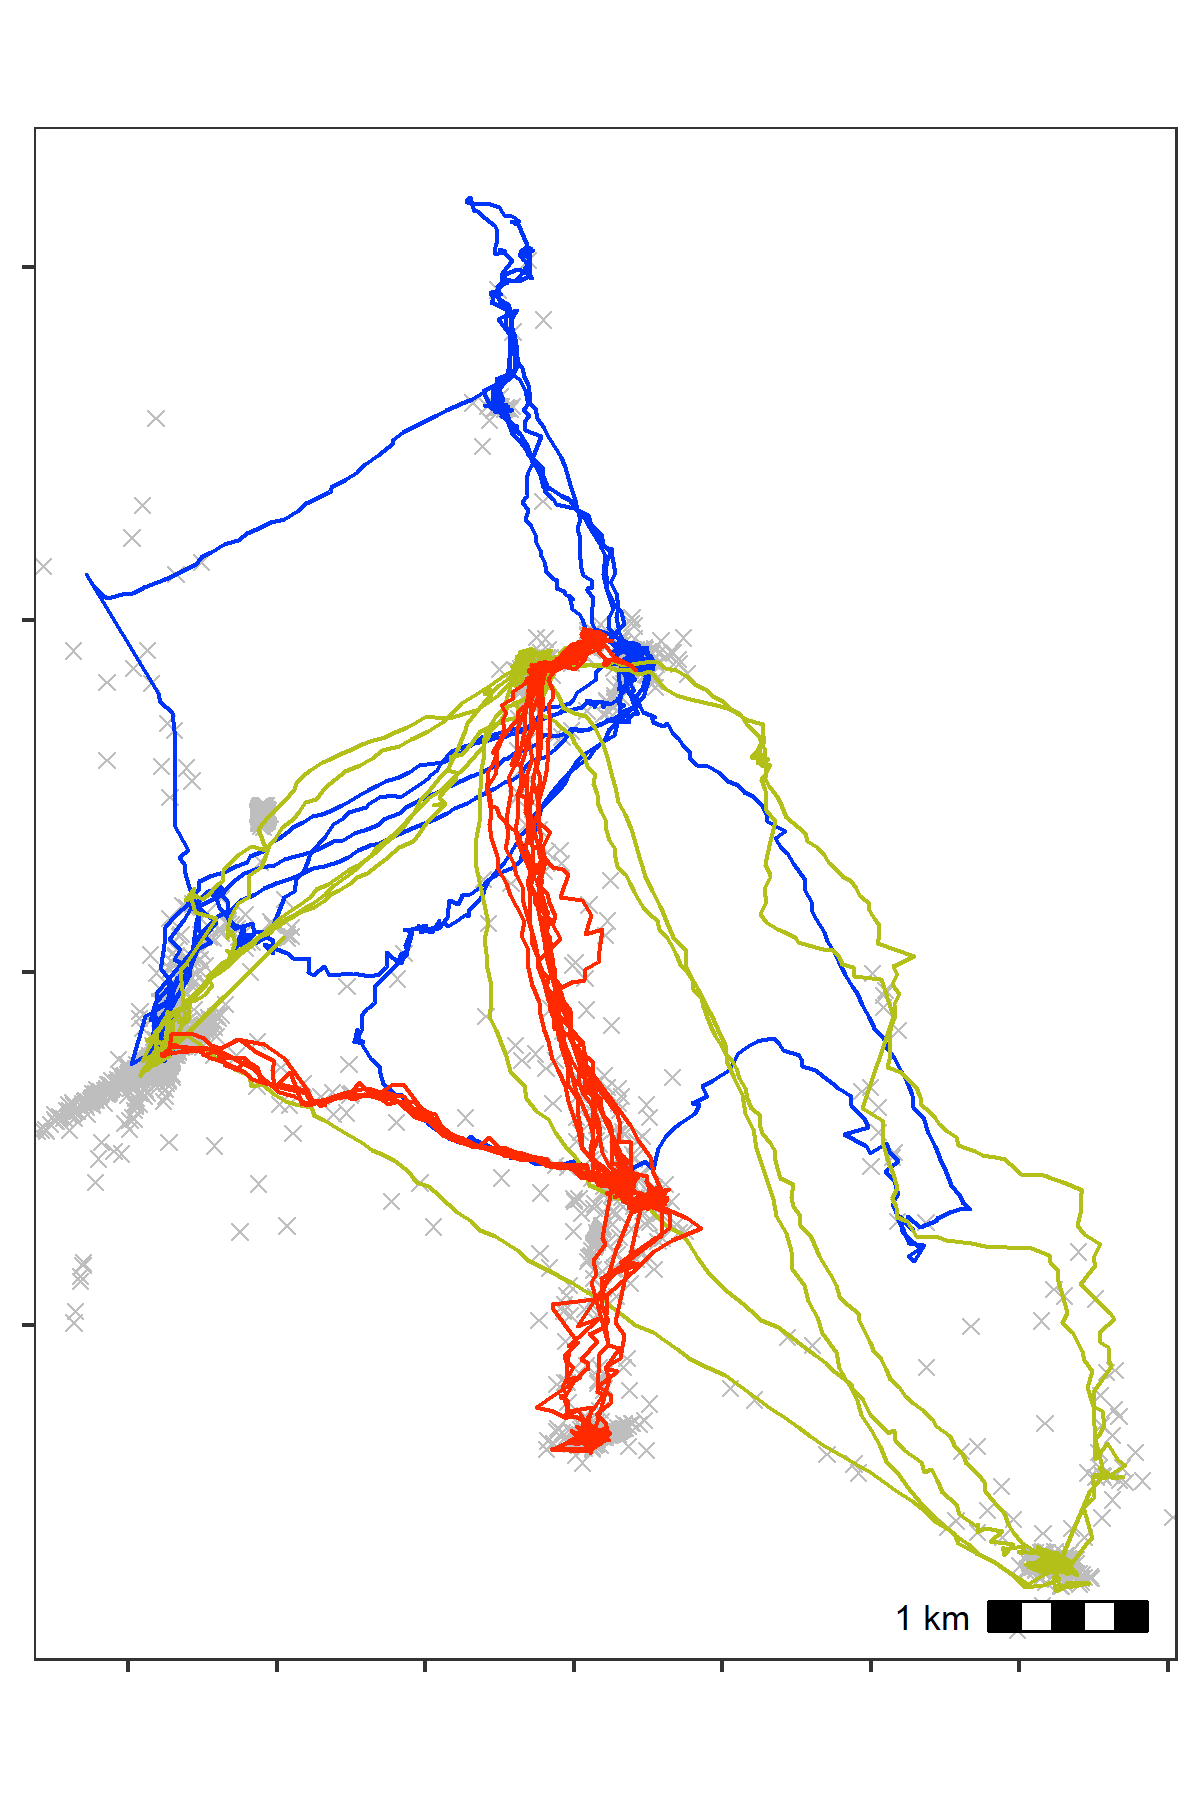
\includegraphics{figures/fig_bat_filter_speed.png}
\caption{Bat data with unrealistic speeds removed. Grey crosses show data that were removed. We calculated the incoming and outgoing speed of each position using \texttt{atl\_get\_speed}, and filtered out positions with speeds \textgreater{} 20 m/s using \texttt{atl\_filter\_covariates}, leaving 10,337 positions per individual on average (98\% from the previous step).}
\end{figure}

\hypertarget{median-smoothing}{%
\subsection{Median smoothing}\label{median-smoothing}}

The quality of this data (Figure 3) is relatively high, and a median smooth is not strictly necessary. We demonstrate the application of a 5 point median smooth to the data nonetheless.

Since the median smoothing function \texttt{atl\_median\_smooth} modifies in place, we first make a copy of the data, using \texttt{data.table}'s \texttt{copy} function.
No reassignment is required, in this case. The \texttt{lapply} function allows arguments to \texttt{atl\_median\_smooth} to be passed within \texttt{lapply} itself.

In this case, the same moving window \(K\) is applied to all individuals, but modifying this code to use the multivariate version \texttt{Map} allows different \(K\) to be used for different individuals. This is a programming matter, and is not covered here further.

\begin{Shaded}
\begin{Highlighting}[]
\CommentTok{\# since the function modifies in place, we shall make a copy}
\NormalTok{data\_smooth <{-}}\StringTok{ }\KeywordTok{copy}\NormalTok{(data\_split)}

\CommentTok{\# split the data again}
\NormalTok{data\_smooth <{-}}\StringTok{ }\KeywordTok{split}\NormalTok{(data\_smooth, }\DataTypeTok{by =} \StringTok{"TAG"}\NormalTok{)}
\end{Highlighting}
\end{Shaded}

\begin{Shaded}
\begin{Highlighting}[]
\CommentTok{\# apply the median smooth to each list element}
\CommentTok{\# no reassignment is required as THE FUNCTION MODIFIES IN PLACE!}
\KeywordTok{invisible}\NormalTok{(}
  
  \CommentTok{\# the function arguments to atl\_median\_smooth}
  \CommentTok{\# can be passed directly in lapply}
  
  \KeywordTok{lapply}\NormalTok{(}\DataTypeTok{X =}\NormalTok{ data\_smooth, }
         \DataTypeTok{FUN =}\NormalTok{ atl\_median\_smooth,}
         \DataTypeTok{time =} \StringTok{"time"}\NormalTok{, }\DataTypeTok{moving\_window =} \DecValTok{5}\NormalTok{)}
\NormalTok{)}
\end{Highlighting}
\end{Shaded}

\hypertarget{sanity-check-plot-smoothed-data}{%
\subsubsection{Sanity check: Plot smoothed data}\label{sanity-check-plot-smoothed-data}}

\begin{figure}
\centering
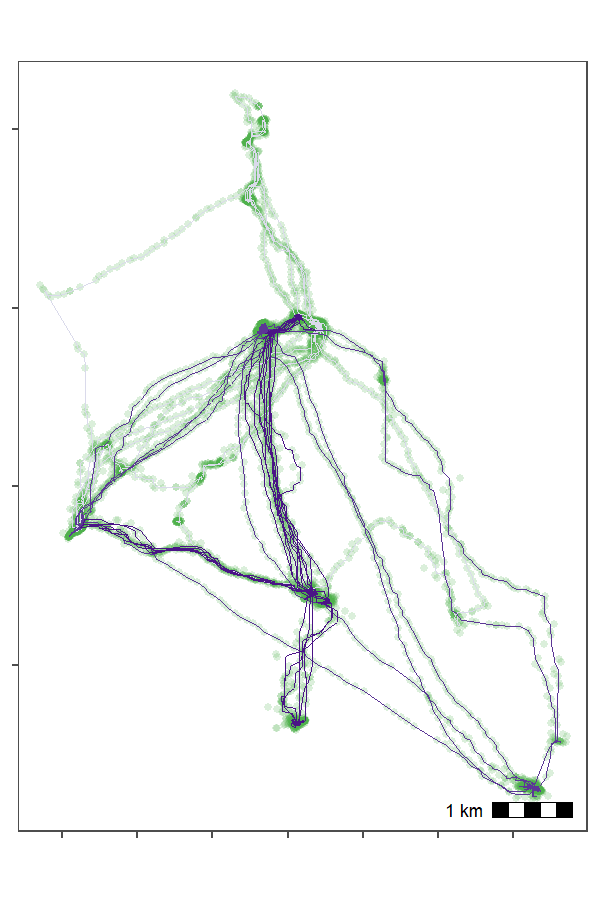
\includegraphics{figures/fig_bat_smooth.png}
\caption{Bat data after applying a median smooth with a moving window \(K\) = 5. Grey crosses show data prior to smoothing. The smoothing step did not discard any data.}
\end{figure}

\hypertarget{making-residence-patches}{%
\subsection{Making residence patches}\label{making-residence-patches}}

\hypertarget{calculating-residence-time}{%
\subsubsection{Calculating residence time}\label{calculating-residence-time}}

First, the data is put through the \texttt{recurse} package to get residence time (Bracis, Bildstein, and Mueller \protect\hyperlink{ref-bracis2018}{2018}).

\begin{Shaded}
\begin{Highlighting}[]
\CommentTok{\# load recurse}
\KeywordTok{library}\NormalTok{(recurse)}

\CommentTok{\# split the data}
\NormalTok{data\_smooth <{-}}\StringTok{ }\KeywordTok{split}\NormalTok{(data\_smooth, data\_smooth}\OperatorTok{$}\NormalTok{TAG)}
\end{Highlighting}
\end{Shaded}

We calculated residence time, but since bats may revisit the same features, we want to prevent confusion between frequent revisits and prolonged residence.

For this, we stop summing residence times within \(Z\) metres of a location if the animal exited the area for one hour or more. The value of \(Z\) (radius, in \texttt{recurse} parameter terms) was chosen as 50m.

This step is relatively complicated and is only required for individuals which frequently return to the same location, or pass over the same areas repeatedly, and for which revisits (cumulative time spent) may be confused for residence time in a single visit.

While a simpler implementation using total residence time divided by the number of revisits is also possible, this does assume that each revisit had the same residence time.

\begin{Shaded}
\begin{Highlighting}[]
\CommentTok{\# get residence times}

\NormalTok{data\_residence <{-}}\StringTok{ }\KeywordTok{lapply}\NormalTok{(data\_smooth, }\ControlFlowTok{function}\NormalTok{(dt) \{}
  \CommentTok{\# do basic recurse}
\NormalTok{  dt\_recurse <{-}}\StringTok{ }\KeywordTok{getRecursions}\NormalTok{(}
    \DataTypeTok{x =}\NormalTok{ dt[, }\KeywordTok{c}\NormalTok{(}\StringTok{"X"}\NormalTok{, }\StringTok{"Y"}\NormalTok{, }\StringTok{"time"}\NormalTok{, }\StringTok{"TAG"}\NormalTok{)],}
    \DataTypeTok{radius =} \DecValTok{50}\NormalTok{,}
    \DataTypeTok{timeunits =} \StringTok{"mins"}
\NormalTok{  )}
  
  \CommentTok{\# get revisit stats}
\NormalTok{  dt\_recurse <{-}}\StringTok{ }\KeywordTok{setDT}\NormalTok{(}
\NormalTok{    dt\_recurse[[}\StringTok{"revisitStats"}\NormalTok{]]}
\NormalTok{  )}
  
  \CommentTok{\# count long absences from the area}
\NormalTok{  dt\_recurse[, timeSinceLastVisit }\OperatorTok{:}\ErrorTok{=}
\StringTok{          }\KeywordTok{ifelse}\NormalTok{(}\KeywordTok{is.na}\NormalTok{(timeSinceLastVisit), }\OperatorTok{{-}}\OtherTok{Inf}\NormalTok{, timeSinceLastVisit)]}
\NormalTok{  dt\_recurse[, longAbsenceCounter }\OperatorTok{:}\ErrorTok{=}\StringTok{ }\KeywordTok{cumsum}\NormalTok{(timeSinceLastVisit }\OperatorTok{>}\StringTok{ }\DecValTok{60}\NormalTok{),}
\NormalTok{             by =}\StringTok{ }\NormalTok{.(coordIdx)}
\NormalTok{             ]}
  \CommentTok{\# get data before the first long absence of 60 mins}
\NormalTok{  dt\_recurse <{-}}\StringTok{ }\NormalTok{dt\_recurse[longAbsenceCounter }\OperatorTok{<}\StringTok{ }\DecValTok{1}\NormalTok{, ]}
  
\NormalTok{  dt\_recurse <{-}}\StringTok{ }\NormalTok{dt\_recurse[, }\KeywordTok{list}\NormalTok{(}
    \DataTypeTok{resTime =} \KeywordTok{sum}\NormalTok{(timeInside),}
    \DataTypeTok{fpt =} \KeywordTok{first}\NormalTok{(timeInside),}
    \DataTypeTok{revisits =} \KeywordTok{max}\NormalTok{(visitIdx)}
\NormalTok{  ),}
\NormalTok{  by =}\StringTok{ }\NormalTok{.(coordIdx, x, y)}
\NormalTok{  ]}
  
  \CommentTok{\# prepare and merge existing data with recursion data}
\NormalTok{  dt[, coordIdx }\OperatorTok{:}\ErrorTok{=}\StringTok{ }\KeywordTok{seq}\NormalTok{(}\KeywordTok{nrow}\NormalTok{(dt))]}
  
\NormalTok{  dt <{-}}\StringTok{ }\KeywordTok{merge}\NormalTok{(dt, }
\NormalTok{              dt\_recurse[, }\KeywordTok{c}\NormalTok{(}\StringTok{"coordIdx"}\NormalTok{, }\StringTok{"resTime"}\NormalTok{)], }
              \DataTypeTok{by =} \KeywordTok{c}\NormalTok{(}\StringTok{"coordIdx"}\NormalTok{))}
  
  \KeywordTok{setorderv}\NormalTok{(dt, }\StringTok{"time"}\NormalTok{)}
\NormalTok{\})}
\end{Highlighting}
\end{Shaded}

We bind the data together and assign a human readable timestamp column.

\begin{Shaded}
\begin{Highlighting}[]
\CommentTok{\# bind the list}
\NormalTok{data\_residence <{-}}\StringTok{ }\KeywordTok{rbindlist}\NormalTok{(data\_residence)}

\CommentTok{\# get time as human readable}
\NormalTok{data\_residence[, ts }\OperatorTok{:}\ErrorTok{=}\StringTok{ }\KeywordTok{as.POSIXct}\NormalTok{(time, }\DataTypeTok{origin =} \StringTok{"1970{-}01{-}01"}\NormalTok{)]}
\end{Highlighting}
\end{Shaded}

\hypertarget{constructing-residence-patches}{%
\subsubsection{Constructing residence patches}\label{constructing-residence-patches}}

Some preparation is required. First, the function requires columns \texttt{x}, \texttt{y},
\texttt{time}, and \texttt{id}, which we assign using the \texttt{data.table} syntax.
Then we subset the data to only work with positions where the individual had a residence time of more than 5 minutes.

\begin{Shaded}
\begin{Highlighting}[]
\CommentTok{\# add an id column}
\NormalTok{data\_residence[, }\StringTok{\textasciigrave{}}\DataTypeTok{:=}\StringTok{\textasciigrave{}}\NormalTok{(}\DataTypeTok{id =}\NormalTok{ TAG,}
                      \DataTypeTok{x =}\NormalTok{ X, }\DataTypeTok{y =}\NormalTok{ Y)]}

\CommentTok{\# filter for residence time > 5 minutes}
\NormalTok{data\_residence <{-}}\StringTok{ }\NormalTok{data\_residence[resTime }\OperatorTok{>}\StringTok{ }\DecValTok{5}\NormalTok{, ]}

\CommentTok{\# split the data}
\NormalTok{data\_residence <{-}}\StringTok{ }\KeywordTok{split}\NormalTok{(data\_residence, data\_residence}\OperatorTok{$}\NormalTok{TAG)}
\end{Highlighting}
\end{Shaded}

We apply the residence patch method, using the default argument values (\texttt{lim\_spat\_indep\ =\ 100} (metres), \texttt{lim\_time\_indep\ =\ 30} (minutes), and \texttt{min\_fixes\ =\ 3}). We change the \texttt{buffer\_radius} to 25 metres (twice the buffer radius is used, so points must be separated by 50m to be independent bouts).

\begin{Shaded}
\begin{Highlighting}[]
\CommentTok{\# segment into residence patches}
\NormalTok{data\_patches <{-}}\StringTok{ }\KeywordTok{lapply}\NormalTok{(data\_residence, atl\_res\_patch,}
                       \DataTypeTok{buffer\_radius =} \DecValTok{25}\NormalTok{)}
\end{Highlighting}
\end{Shaded}

\hypertarget{getting-residence-patch-data}{%
\subsubsection{Getting residence patch data}\label{getting-residence-patch-data}}

We extract the residence patch data as spatial \texttt{sf-MULTIPOLYGON} objects.
These are returned as a list and must be converted into a single \texttt{sf} object.
These objects and the raw movement data are shown in Figure 5.

\begin{Shaded}
\begin{Highlighting}[]
\CommentTok{\# get data spatials}
\NormalTok{data\_spatials <{-}}\StringTok{ }\KeywordTok{lapply}\NormalTok{(data\_patches, atl\_patch\_summary,}
                        \DataTypeTok{which\_data =} \StringTok{"spatial"}\NormalTok{,}
                        \DataTypeTok{buffer\_radius =} \DecValTok{25}\NormalTok{)}

\CommentTok{\# bind list}
\NormalTok{data\_spatials <{-}}\StringTok{ }\KeywordTok{rbindlist}\NormalTok{(data\_spatials)}

\CommentTok{\# convert to sf}
\KeywordTok{library}\NormalTok{(sf)}
\NormalTok{data\_spatials <{-}}\StringTok{ }\KeywordTok{st\_sf}\NormalTok{(data\_spatials, }\DataTypeTok{sf\_column\_name =} \StringTok{"polygons"}\NormalTok{)}

\CommentTok{\# assign a crs}
\KeywordTok{st\_crs}\NormalTok{(data\_spatials) <{-}}\StringTok{ }\KeywordTok{st\_crs}\NormalTok{(}\DecValTok{2039}\NormalTok{)}
\end{Highlighting}
\end{Shaded}

\hypertarget{write-patch-spatial-representations}{%
\subsubsection{Write patch spatial representations}\label{write-patch-spatial-representations}}

\begin{Shaded}
\begin{Highlighting}[]
\KeywordTok{st\_write}\NormalTok{(data\_spatials,}
         \DataTypeTok{dsn =} \StringTok{"data/data\_bat\_residence\_patches.gpkg"}\NormalTok{)}
\end{Highlighting}
\end{Shaded}

Write cleaned bat data.

\begin{Shaded}
\begin{Highlighting}[]
\NormalTok{data\_clean <{-}}\StringTok{ }\KeywordTok{fwrite}\NormalTok{(}\KeywordTok{rbindlist}\NormalTok{(data\_smooth),}
                     \DataTypeTok{file =} \StringTok{"data/data\_bat\_smooth.csv"}\NormalTok{)}
\end{Highlighting}
\end{Shaded}

Write patch summary.

\begin{Shaded}
\begin{Highlighting}[]
\CommentTok{\# get summary}
\NormalTok{patch\_summary <{-}}\StringTok{ }\KeywordTok{lapply}\NormalTok{(data\_patches, atl\_patch\_summary)}

\CommentTok{\# bind summary}
\NormalTok{patch\_summary <{-}}\StringTok{ }\KeywordTok{rbindlist}\NormalTok{(patch\_summary)}

\CommentTok{\# write}
\KeywordTok{fwrite}\NormalTok{(patch\_summary,}
       \StringTok{"data/data\_bat\_patch\_summary.csv"}\NormalTok{)}
\end{Highlighting}
\end{Shaded}

\begin{figure}
\centering
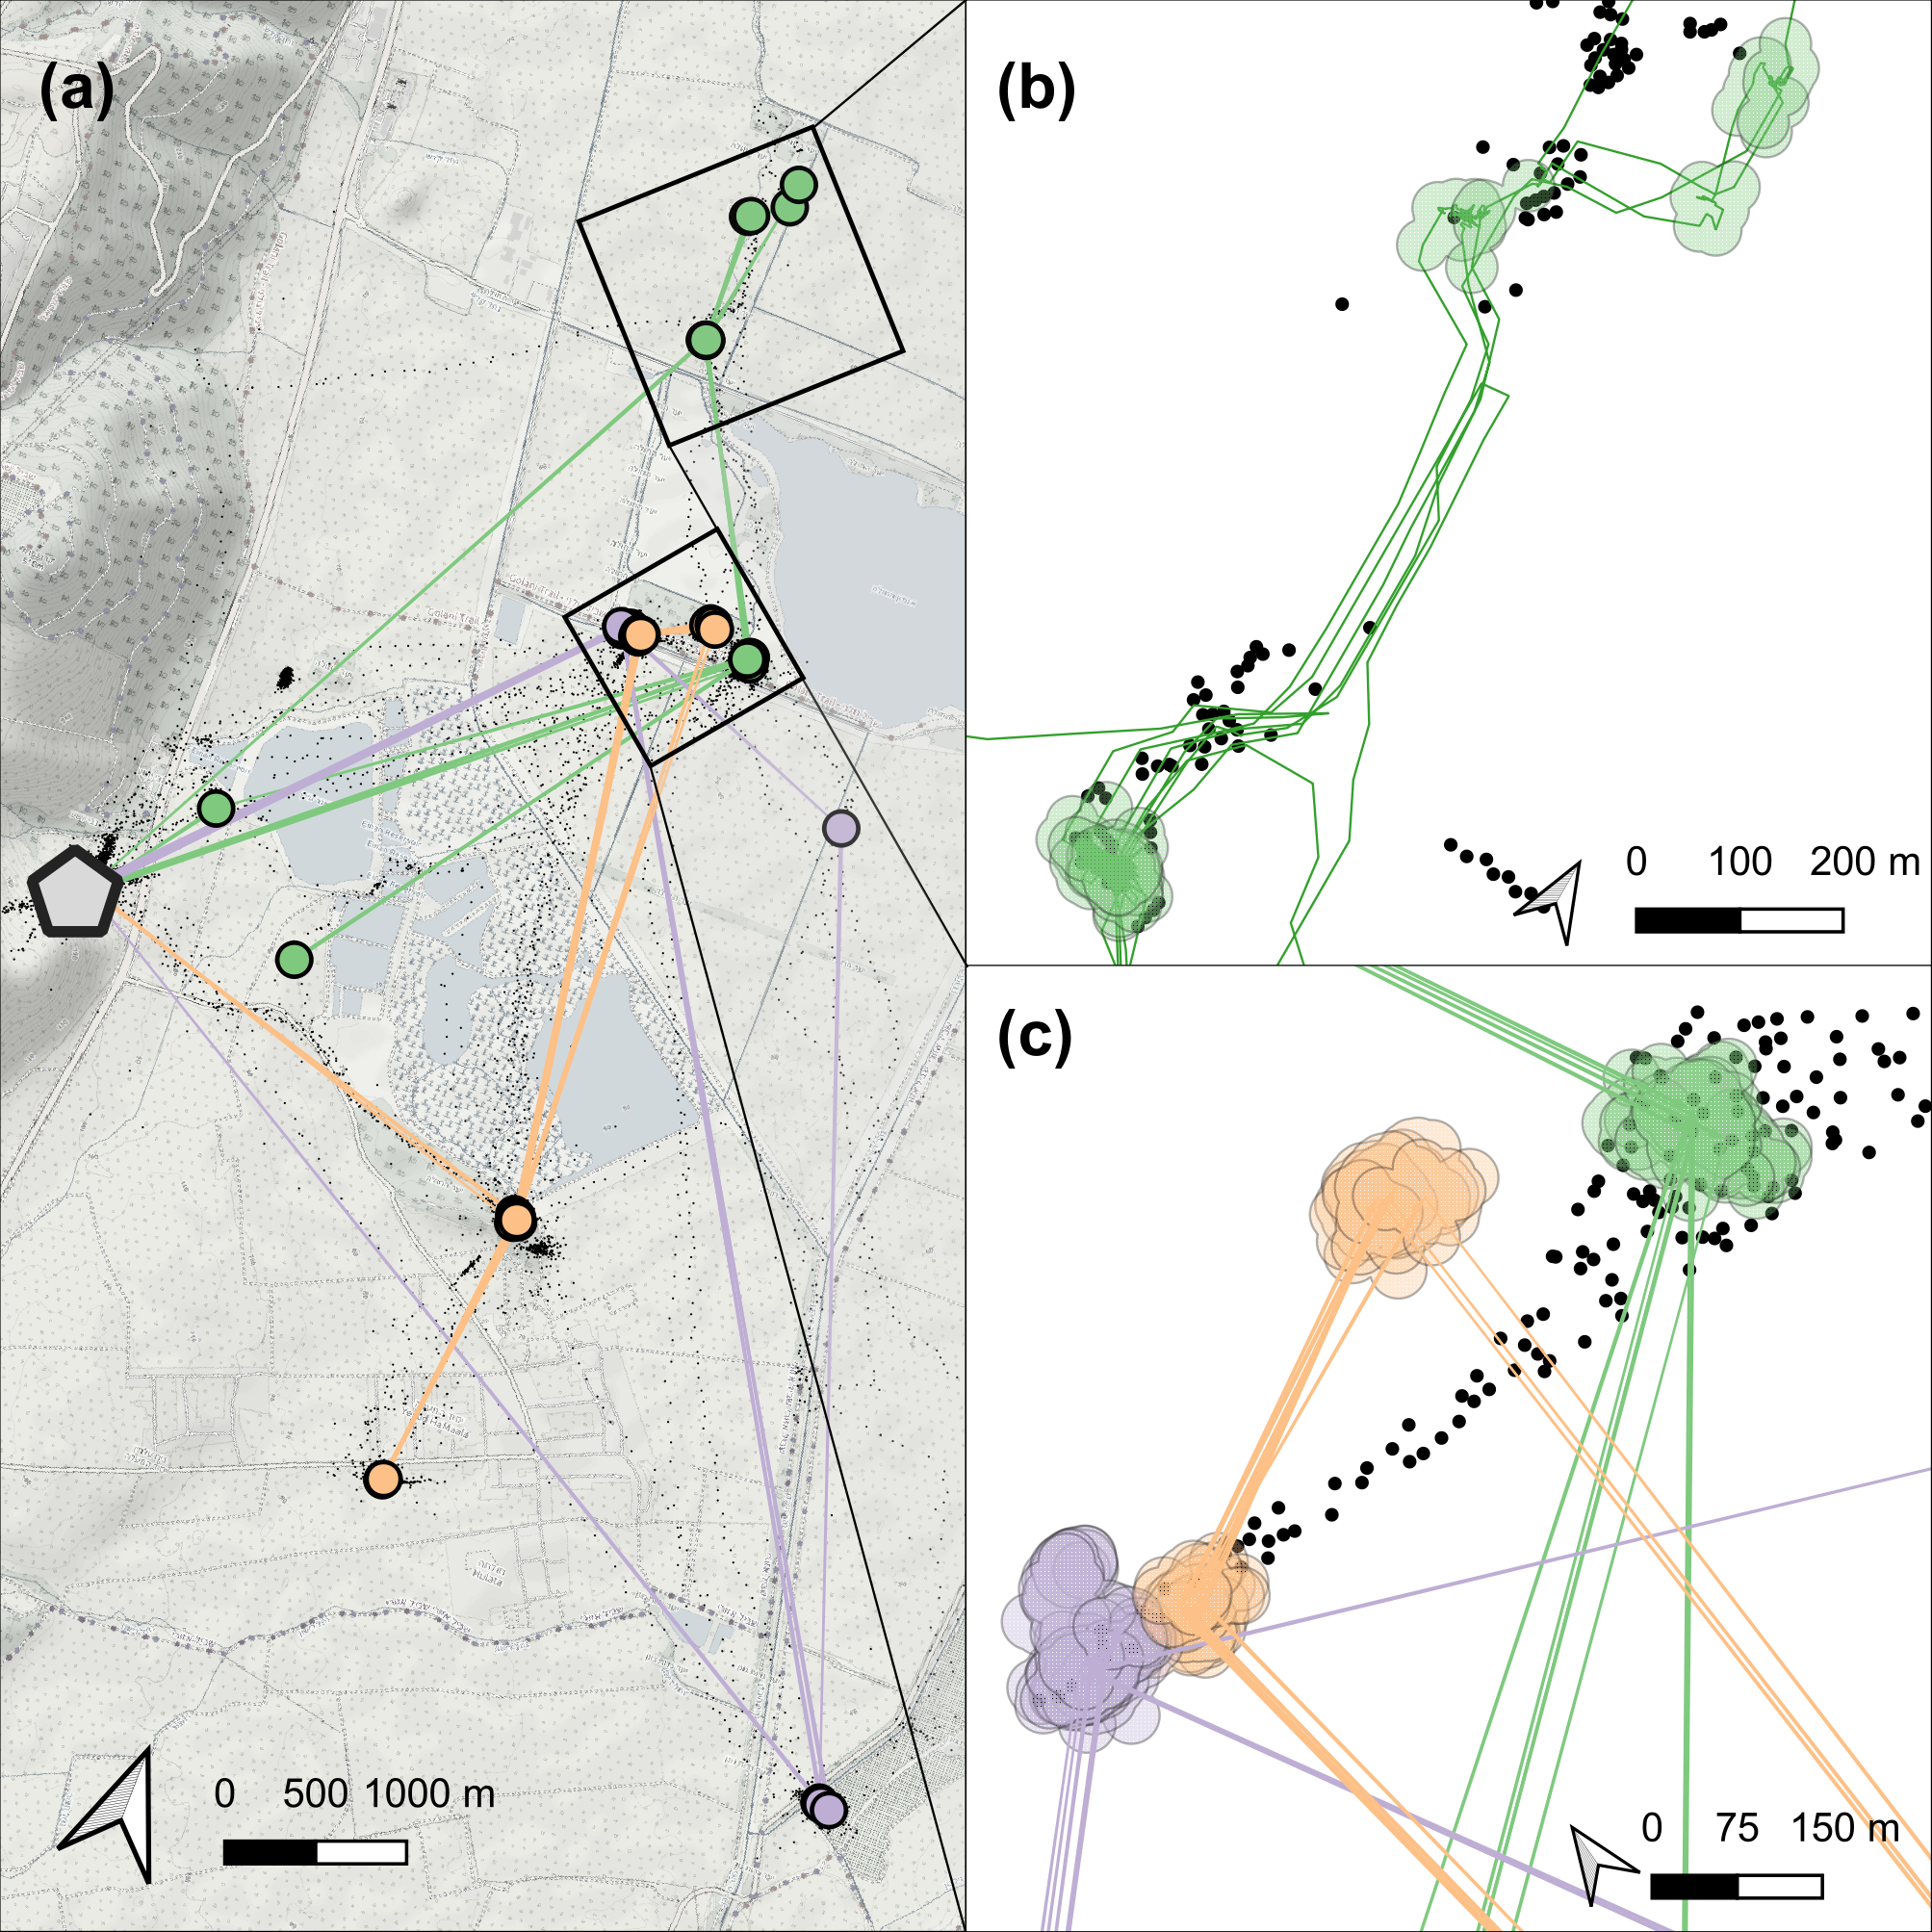
\includegraphics{figures/fig_bat_patches.png}
\caption{A visual examination of plots of the bats' residence patches and linear approximations of paths between them showed that though all three bats roosted at the same site, they used distinct areas of the study site over the three nights \textbf{(a)}.
Bats tended to be resident near fruit trees, which are their main food source, travelling repeatedly between previously visited areas \textbf{(b, c)}.
However, bats also appeared to spend some time at locations where no fruit trees were recorded, prompting questions about their use of other food sources \textbf{(b, c)}.
When bats did occur close together, their residence patches barely overlapped, and their paths to and from the broad area of co-occurrence were not similar \textbf{(c)}.
Constructing residence patches for multiple individuals over multiple activity periods suggests interesting dynamics of within- and between-individual overlap \textbf{(b, c)}.}
\end{figure}

\hypertarget{references}{%
\section{References}\label{references}}

\hypertarget{refs}{}
\begin{cslreferences}
\leavevmode\hypertarget{ref-bracis2018}{}%
Bracis, Chloe, Keith L. Bildstein, and Thomas Mueller. 2018. ``Revisitation Analysis Uncovers Spatio-Temporal Patterns in Animal Movement Data.'' \emph{Ecography} 41 (11): 1801--11. \url{https://doi.org/10.1111/ecog.03618}.

\leavevmode\hypertarget{ref-dowle2020}{}%
Dowle, Matt, and Arun Srinivasan. 2020. \emph{Data.Table: Extension of `data.Frame`}. Manual.

\leavevmode\hypertarget{ref-gupte2020a}{}%
Gupte, Pratik Rajan. 2020. ``Atlastools: Pre-Processing Tools for High Frequency Tracking Data.'' Zenodo. \url{https://doi.org/10.5281/ZENODO.4033154}.

\leavevmode\hypertarget{ref-shohami2020}{}%
Shohami, David, and Ran Nathan. 2020. ``Cognitive Map-Based Navigation in Wild Bats Revealed by a New High-Throughput Tracking System.'' Dryad. \url{https://doi.org/10.5061/DRYAD.G4F4QRFN2}.

\leavevmode\hypertarget{ref-toledo2020}{}%
Toledo, Sivan, David Shohami, Ingo Schiffner, Emmanuel Lourie, Yotam Orchan, Yoav Bartan, and Ran Nathan. 2020. ``Cognitive MapBased Navigation in Wild Bats Revealed by a New High-Throughput Tracking System.'' \emph{Science} 369 (6500): 188--93. \url{https://doi.org/10.1126/science.aax6904}.

\leavevmode\hypertarget{ref-weiser2016}{}%
Weiser, Adi Weller, Yotam Orchan, Ran Nathan, Motti Charter, Anthony J. Weiss, and Sivan Toledo. 2016. ``Characterizing the Accuracy of a Self-Synchronized Reverse-GPS Wildlife Localization System.'' In \emph{2016 15th ACM/IEEE International Conference on Information Processing in Sensor Networks (IPSN)}, 1--12. \url{https://doi.org/10.1109/IPSN.2016.7460662}.
\end{cslreferences}

\end{document}
